\documentclass{article}
\usepackage[utf8]{inputenc}
\usepackage{fontspec}
\usepackage{tabularx}
\usepackage{bbding}
\setmainfont[
  Path = ./,
  Ligatures = TeX,
  BoldFont = SABONLTSTD-BOLD.OTF,
  ItalicFont = SABONLTSTD-ITALIC.OTF,
]{SABONLTSTD-ROMAN.OTF}
\usepackage{book-of-common-prayer}
\geometry{
  paperheight=8.5in,
  paperwidth=5.5in,
  heightrounded,
}

\newwrite\dimensionout
\immediate\openout\dimensionout=linewidth.txt
\immediate\write\dimensionout{\the\linewidth}
\immediate\closeout\dimensionout

\title{An Order for\\COMPLINE\\\quad\\\footnotesize{From the
\textit{Anglican Service Book}}}
\author{}

\begin{document}
\maketitle

\newpage

\section*{Preface}

In the following is an adaptation of the \textit{Compline} service from
the \textit{Anglican Service Book}, which is an adaptation of the
Rite II services from the Book of Common Prayer (1979) to a Rite I language.
In the following, I have taken the liberty of including more options from the
Compline of the Book of Common Prayer (1979), as well as some notes from the
Anglican Breviary. Specifically:
\begin{enumerate}
  \item Additional Brief Lessons;
  \item Instructions from the Anglican Breviary;
  \item Additional instructions to break up the text a little bit more
    (these are my personal opinions, presented as if they were real
      instructions;
    I won't mark them);
  \item Music for the Psalms, where \textbf{bold} indicates the note which one
    comes off from the monotone, the \underline{underline} denotes
    sharing the same
    tone for both syllables, the accént indicating a shift in the
    mediation after
    the principal shift, and the ümlaut indicates a \textit{pes} or
    \textit{clivis}.
  \item Additional collects, with minimal changes (you to thee, and
    your to thy/thine)
\end{enumerate}

This project is a personal project, created as a hobby.

\newpage

\section*{Compline}

\instruct{The Officiant begins:}

\begin{tabularx}{\linewidth}{lX}
  & \CrossMaltese~The Lord Almighty grant us a quiet night and a perfect end. \\
  \textit{People} & \textbf{Amen.}
\end{tabularx}

\section*{Brief Lesson}

\instruct{Then the Officiant reads one of the following Brief Lessons}

\bibleverse
{Be Sober, be vigilant, because your adversary the devil, as a
  roaring lion, walketh about, seeking whom he may devour: whom resist,
steadfast in the faith. But thou, O Lord, have mercy upon us.}
{1 Peter 5:8-9a}

\begin{tabularx}{\linewidth}{lX}
  \textit{People} & \textbf{Thanks be to God.}
\end{tabularx}

\instruct{or}

\bibleverse
{Now the God of peace, that brought again from the dead our Lord Jesus,
  that great shepherd of the sheep, through the blood of the
  everlasting covenant,
  make you perfect in every good work to do his will, working in you that
  which is well-pleasing in his sight, through Jesus Christ; to whom be
glory for ever and ever. Amen.}
{Hebrews 13:20-21}

\begin{tabularx}{\linewidth}{lX}
  \textit{People} & \textbf{Thanks be to God.}
\end{tabularx}

\instruct{or}

\bibleverse
{Come unto me, all ye that labour and are heavy laden, and I will give you
  rest. Take my yoke upon you, and learn of me; for I am meek and
  lowly in heart: and ye shall find rest unto your souls.
For my yoke is easy, and my burden is light.}
{Matthew 11:28-30}

\begin{tabularx}{\linewidth}{lX}
  \textit{People} & \textbf{Thanks be to God.}
\end{tabularx}

\instruct{or}

\bibleverse
{Thou, O \textsc{Lord}, art in the midst of us, and we are called by
thy name; leave us not, O \textsc{Lord} our God.}
{Jeremiah 14:9, 22}

\begin{tabularx}{\linewidth}{lX}
  \textit{People} & \textbf{Thanks be to God.}
\end{tabularx}

\section*{Confession}

\begin{tabularx}{\linewidth}{lX}
  \textit{Officiant} & Our help \CrossMaltese~is in the name of the Lord. \\
  \textit{People} & \textbf{Who hath made heaven and earth.} \\
  \textit{Officiant} & Let us humbly confess our sins unto Almighty God. \\
\end{tabularx}

\instruct{Then the Our Father is said secretly. All then say,}
\newline
\begin{prayer}
  Almighty God, our heavenly Father:
  We have sinned against thee,
  through our own fault,
  in thought word and deed,
  and in those things we have left undone.
  For the sake of thy Son our Lord Jesus Christ,
  forgive us all our offenses;
  And grant that we may serve thee in newness of life,
  to the glory of thy Name. Amen.

\end{prayer}

\instruct{Then the Officiant says}

\begin{tabularx}{\linewidth}{lX}
  & The almighty God grant us \CrossMaltese~forgiveness of all our sins,
  amendment of life, and the grace and comfort of the Holy Ghost. \\
  \textit{People} & \textbf{Amen.}
\end{tabularx}

\section*{The Psalms}

\instruct{The Opening Versicles are then said, followed by the Gloria}

\begin{tabularx}{\linewidth}{lX}
  \textit{Officiant} & O God, make speed to save us.  \\
  \textit{People} & \CrossMaltese~\textbf{O Lord, make haste to help us.}\\
  & \\
  \textit{Officiant} & Glory be to the Father, and to the Son, and to
  the Holy Ghost.  \\
  \textit{People} & \textbf{As it was in the beginning, is now, and
  ever shall be, world without end. Amen.}
\end{tabularx}

\instruct{Then shall be sung or said one or more of the following Psalms, or
any other suitable Psalms.}

\newpage
\subsection*{Psalm 4\quad Cum invocarem}

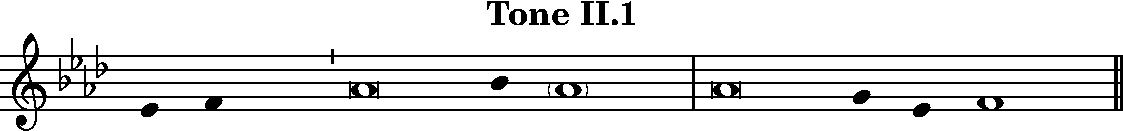
\includegraphics[width=\linewidth]{./psalms/psalm4-crop.pdf}

\begin{enumerate}[
      leftmargin=*,
      label=\textsc { \arabic * }
    ]
  \item \psalmverse{ \textsc{Hear me} when I call, O God of my
    \textbf{righ}-\underline{teous-ness:} }
    {thou hast set me at liberty when I was in trouble; have mercy
    upon me, and hearken un-\textbf{to} my prayer.}

  \item \psalmverse{O ye sons of men, how long will ye blaspheme mine
    \textbf{hon}-our:}
    {and have such pleasure in vanity, and seek af-\textbf{ter} false-hood?}

  \item \psalmverse{Know this also, that the Lord hath chosen to
    himself the man that is \textbf{god}-ly:}
    {when I call upon the Lord, he \textbf{will} hear me.}

  \item \psalmverse{Stand in awe, and \textbf{sin} not:}
    {commune with your own heart, and in your cham-\textbf{ber},
    \underline{and be} still.}

  \item \psalmverse{Offer the sacrifice of
    \textbf{righ}-\underline{teous-ness:}}
    {and put your trust \textbf{in} the Lord.}

  \item \psalmverse{There be many that say, `Who will show us any
    \textbf{good}?':}
    {Lord, lift thou up the light of thy countenance \textbf{up}-on us.}

  \item \psalmverse{Thou hast put gladness in my \textbf{heart}:}
    {more than men have when their grain \textbf{and}
    \underline{wine in}-crease.}

  \item \psalmverse{I will lay me down in peace, and take my \textbf{rest}:}
    {for it is thou, Lord, only, that makest me dwell \textbf{in} safe-ty.}

  \item[] \psalmverse{Glory be to the Father, and to the \textbf{Son}:}
    {and to \textbf{the} \underline{Ho-ly} Ghost;}

  \item[] \psalmverse{As it was in the beginning, is now, and ever
    \textbf{shall} be:}
    {world without \textbf{end}. A-men.}
\end{enumerate}

\subsection*{Psalm 31:1-6\quad In te, Domine, speravi}

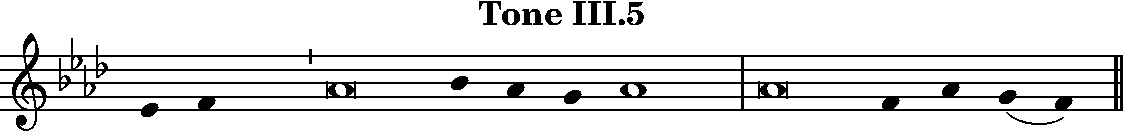
\includegraphics[width=\linewidth]{./psalms/psalm31-crop.pdf}

\begin{enumerate}[
      leftmargin=*,
      label=\textsc { \arabic *}
    ]

  \item \psalmverse{\textsc{In thee}, O Lord, \textbf{have}
    \underline{I put} my trust:}
    {let me never be put to confusion, deliver me in \textbf{thy}
    \underline{righ-teous}-nëss.}

  \item \psalmverse{Bow \textbf{down} \underline{thine ear} to me:}
    {make haste to \textbf{de}-\underline{liv-er} më.}

  \item \psalmverse{And be thou my strong rock, and \textbf{house} of de-fence:}
    {that thou may-\textbf{est} save më.}

  \item \psalmverse{For thou art my strong rock, \textbf{and} my cas-tle:}
    {be thou also my guide, and lead me for \textbf{thy} Name's säke.}

  \item \psalmverse{Draw me out of the net that they have
    \textbf{hid}-den for me:}
    {for thou \textbf{art} my strëngth.}

  \item \psalmverse{Into thy hands I com-\textbf{mend} my spi-rit:}
    {for thou hast redeemèd me, O Lord, \textbf{thou} \underline{God
    of} trüth.}

  \item[] \psalmverse{Glory be to the Father, \textbf{and} to the Son:}
    {and to \textbf{the} \underline{Ho-ly} Ghöst;}

  \item[] \psalmverse{As it was in the beginning, is now, and
    \textbf{ev}-er shall be:}
    {world without \textbf{end}. A-men.}

\end{enumerate}

\subsection*{Psalm 91\quad Qui habitat}

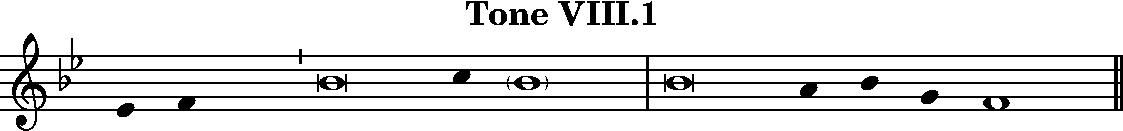
\includegraphics[width=\linewidth]{psalms/psalm91-crop.pdf}

\begin{enumerate}[
      leftmargin=*,
      label=\textsc{ \arabic * }
    ]
  \item \psalmverse{\textsc{Who-so} dwelleth under the defence of the
    Most \textbf{High}:}
    {shall abide under the shadow of \textbf{the} Al-migh-ty.}

  \item \psalmverse{I will say unto the Lord, `Thou art my refuge and
    my \textbf{strong}-hold:}
    {my God in \textbf{whom} I will trust'.}

  \item \psalmverse{For he shall deliver thee from the snare of the
    \textbf{hun}-ter:}
    {and from the \textbf{noi}-some pes-\underline{ti-lence}.}

  \item \psalmverse{He shall defend thee under his wings, and thou
    shalt be safe under his \textbf{fea}-thers:}
    {his faithfulness is a \textbf{shield} and buck-ler.}

  \item \psalmverse{Thou shalt not be afraid for any terror by \textbf{night}:}
    {nor for the arrow that \textbf{fli}-eth by day;}

  \item \psalmverse{For the pestilence that walketh in \textbf{dark}-ness:}
    {nor for the sickness that destroyeth \textbf{in} the noon-day.}

  \item \psalmverse{A thousand shall fall beside thée, and ten
    thousand at thy right \textbf{hand}:}
    {but it shall \textbf{not} come nigh thee.}

  \item \psalmverse{Yea, with thine eyes shalt thou be-\textbf{hold}:}
    {and see the reward of \textbf{the} un-god-ly.}

  \item \psalmverse{Because thou hast said, `The Lord is my \textbf{re}-fuge':}
    {and hast made the Most High thy \textbf{hab}-i-ta-tion,}

  \item \psalmverse{There shall no evil happen unto \textbf{thee}:}
    {neither shall any plague come \textbf{nigh} thy dwelling.}

  \item \psalmverse{For he shall give his angels charge over \textbf{thee}:}
    {to keep \textbf{thee} in all \underline{thy ways}.}

  \item \psalmverse{They shall bear thee in their \textbf{hands}:}
    {that thou hurt not thy \textbf{foot} a-gainst a stone.}

  \item \psalmverse{Thou shalt go upon the lion and \textbf{ad}-der:}
    {the young lion and the dragon shalt thou tread \textbf{un}-der thy feet.}

  \item \psalmverse{Because he hath set his love upon mé, therefore
    will I de-\textbf{liv}-\underline{er him}:}
    {I will set him up, because \textbf{he} hath known \underline{my Name}.}

  \item \psalmverse{He shall call upon me, and I will \textbf{hear} him:}
    {yea, I am with him in trouble; I will deliver him, and bring
    \textbf{him} to hon-our.}

  \item \psalmverse{With long life will I satisfy \textbf{him}:}
    {and show him \textbf{my} sal-va-tion.}

  \item[] \psalmverse{Glory be to the Father, and to the \textbf{Son}:}
    {and \textbf{to} the \underline{Ho-ly} Ghost;}

  \item[] \psalmverse{As it was in the beginning, is now, and ever
    \textbf{shall} be:}
    {world with-\textbf{out} end. A-men.}

\end{enumerate}

\subsection*{Psalm 134\quad Ecce nunc}

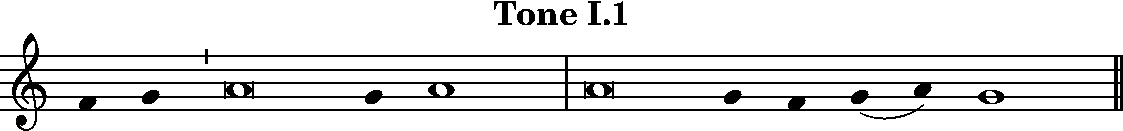
\includegraphics[width=\linewidth]{psalms/psalm134-crop.pdf}

\begin{enumerate}[
      leftmargin=*,
      label=\textsc{ \arabic * }
    ]

  \item \psalmverse{\textsc{Be-hold} now, praise \textbf{the} Lord:}
    {all ye \textbf{ser}-vants öf \underline{the Lord};}

  \item \psalmverse{Ye that by night stand in the house of \textbf{the} Lord:}
    {even in the courts of the \textbf{house} of oür God.}

  \item \psalmverse{Lift up your hands in the sanctu-\textbf{a}-ry:}
    {\textbf{and} präise \underline{the Lord}.}

  \item \psalmverse{The Lord that made heaven \textbf{and} earth:}
    {give thee blessing \textbf{out} of Sï-on.}

  \item[] \psalmverse{Glory be to the Father, and to \textbf{the} Son:}
    {and \textbf{to} the Hö-\underline{ly Ghost};}

  \item[] \psalmverse{As it was in the beginning, is now, and ever
    \textbf{shall} be:}
    {world with-\textbf{out} end. Ä-men.}

\end{enumerate}

\section*{The Hymn}

\instruct{The following hymn is always used, unless otherwise
specified in the Proper}

\subsection*{Te lucis ante terminum}

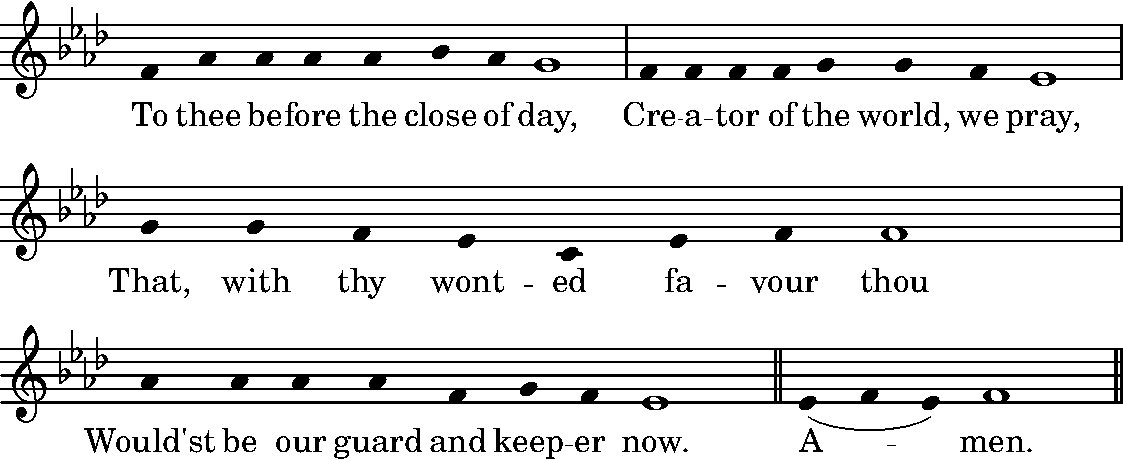
\includegraphics[width=\textwidth]{hymns/telucis-crop.pdf}

\begin{tabularx}{\linewidth}{lX}
  \textbf{1.} & From all ill dreams defend our eyes, \\
  & From nightly fears and fantasies; \\
  & Tread underfoot our ghostly foe, \\
  & That no pollution we may know. \\
  & \\
  \textbf{2.} & O Father, that we ask be done, \\
  & Through Jesus Christ, thine only son; \\
  & Who, with the Holy Ghost and thee, \\
  & Doth live and reign eternally. Amen.
\end{tabularx}

\section*{The Brief Respond}

\subsection*{In manus tuas}

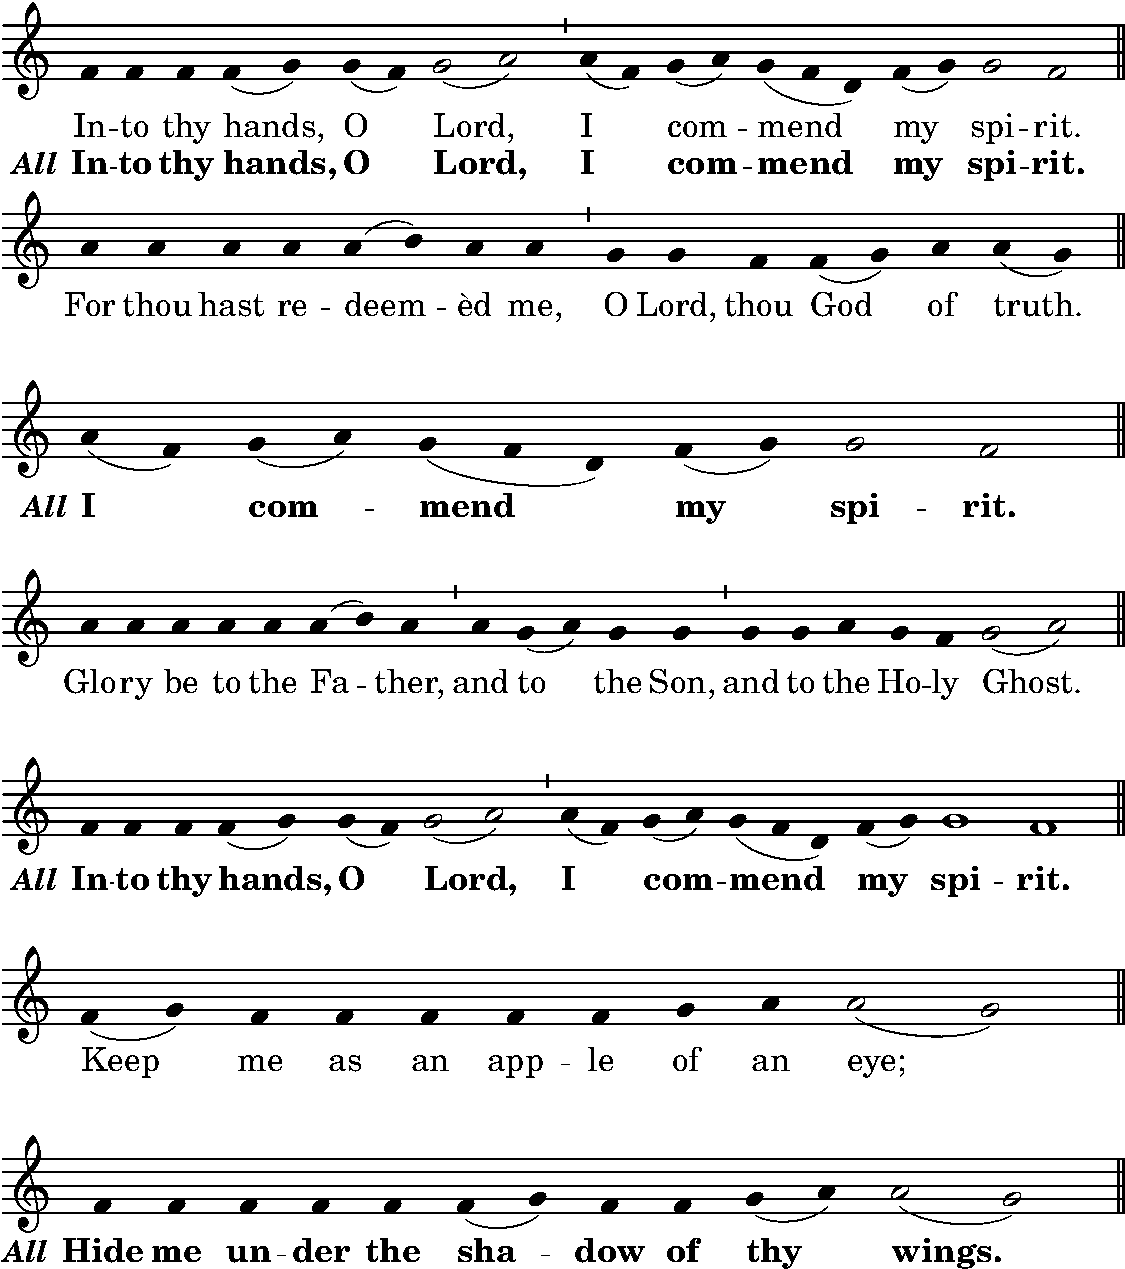
\includegraphics[width=\linewidth]{hymns/intothy-crop.pdf}

\newpage
\section*{Prayers and Intercessions}

\instruct{Then follows}

\begin{tabularx}{\linewidth}{lX}
  \textit{Officiant} & Lord have mercy upon us. \\
  \textit{All} & \textbf{Christ have mercy upon us.} \\
  \textit{Officiant} & Lord have mercy upon us. \\
  & \\
  \textit{All} & \textbf{Our Father, who art in heaven,} \\
  & \textbf{hallowed be thy Name;} \\
  & \textbf{thy kingdom come;} \\
  & \textbf{thy will be done;} \\
  & \textbf{on earth as it is in heaven.} \\
  & \textbf{Give us this day our daily bread.} \\
  & \textbf{And forgive our trespasses,} \\
  & \textbf{as we forgive them that trespass against us.} \\
  & \textbf{And lead us not into temptation;} \\
  & \textbf{but deliver us from evil. Amen.} \\
  & \\
  \textit{Officiant} & O Lord, hear my prayer; \\
  \textit{All} & \textbf{and let my cry come unto thee.}
\end{tabularx}

\instruct{The Officiant then says one of the following Collects}

Visit, we beseech thee, O Lord, this habitation: Drive far from it all snares
of the enemy; let thy holy angels dwell herein to preserve us in peace, and
let thy blessing be ever upon us. Through Jesus Christ our Lord.

\begin{tabularx}{\linewidth}{lX}
  \textit{People} & \textbf{Amen.}
\end{tabularx}

\instruct{or}

Be our light in the darkness, O Lord, and in thy great mercy defend us from all
perils and dangers of this night. For the love of thy only Son, our Savior
Jesus Christ.

\begin{tabularx}{\linewidth}{lX}
  \textit{People} & \textbf{Amen.}
\end{tabularx}

\instruct{or}

Be present, O merciful God, and protect us through the hours of this
night, that we who are wearied by the changes and chances of this life
may rest in thy eternal changelessness. Through Jesus Christ our Lord.

\begin{tabularx}{\linewidth}{lX}
  \textit{People} & \textbf{Amen.}
\end{tabularx}

\instruct{or}

Look down, O Lord, from thy heavenly throne, and illumine this night
with thy celestial brightness; that by night as by day thy people may glorify
thy holy Name. Through Jesus Christ our Lord.

\begin{tabularx}{\linewidth}{lX}
  \textit{People} & \textbf{Amen.}
\end{tabularx}

\instruct{or, a Collect for Saturdays}

We give thanks, O God, for revealing thy Son Jesus Christ
to us by the light of his resurrection: Grant that as we sing thy glory
at the close of this day, our joy may abound in the morning as we celebrate
the Paschal mystery. Through Jesus Christ our Lord.

\begin{tabularx}{\linewidth}{lX}
  \textit{People} & \textbf{Amen.}
\end{tabularx}

\instruct{Silence is kept, intercessions and thanksgivings may be offered.}

\section*{Conclusion}

\instruct{The service ends with the Nunc dimittis and antiphon:}

\subsection*{Antiphon: Salva nos}

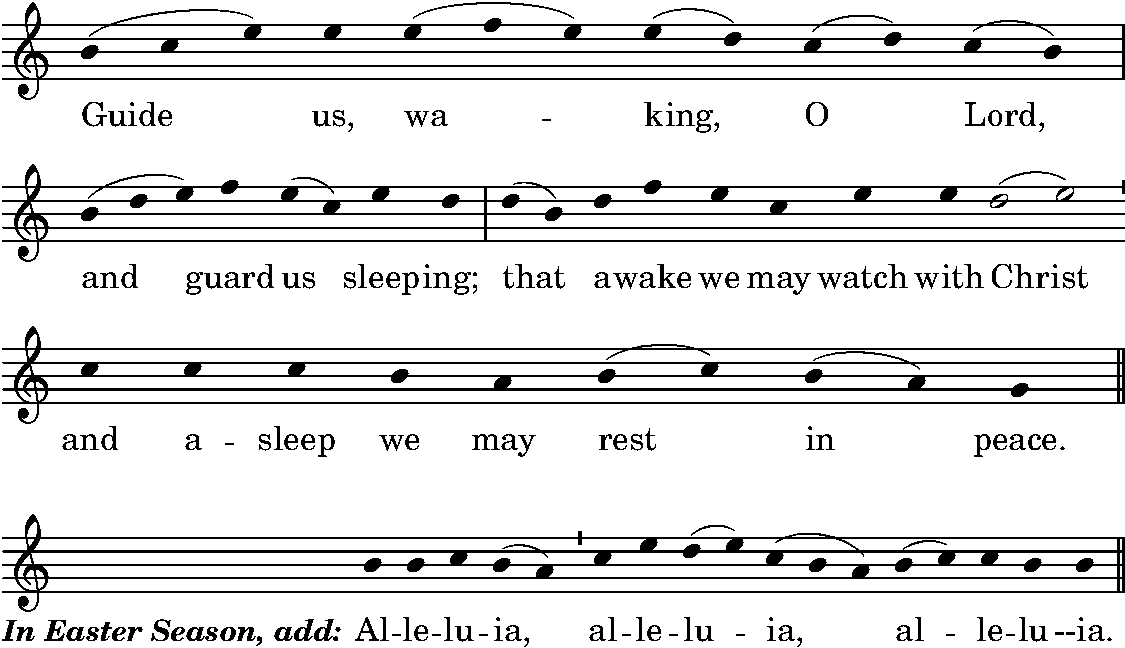
\includegraphics[width=\linewidth]{hymns/guideus-crop.pdf}

\newpage

\subsection*{Nunc dimittis}

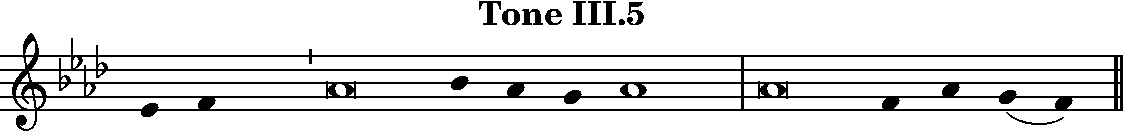
\includegraphics[width=\linewidth]{psalms/psalm31-crop.pdf}

\begin{enumerate}[
      leftmargin=*,
      label=\textsc{\arabic *}
    ]
  \item \psalmverse{\textsc{Lord, now} lettest thou thy
    ser-\textbf{vant} \underline{de-part} ïn peace:}
    {according \textbf{to} thy wörd.}

  \item \psalmverse{\textsc{For mine} eyes have seen \textbf{thy} sal-vä-tion:}
    {which thou hast preparèd before the face of \textbf{all} peo-plë;}

  \item \psalmverse{\textsc{To be} a light to light-\textbf{en} the Gën-tiles:}
    {and to be the glory of thy peo-\textbf{ple} \underline{Is-ra}-ël.}

  \item[] \psalmverse{\textsc{Glo-ry} be to the Father, \textbf{and}
    to thë Son:}
    {and to \textbf{the} \underline{Ho-ly} Ghöst.}

  \item[] \psalmverse{\textsc{As it was} in the beginning, is now,
    and \textbf{ev}-er shäll be:}
    {world without \textbf{end}. A-mën.}
\end{enumerate}

\instruct{Repeat the antiphon, Salva nos}

\begin{tabularx}{\linewidth}{lX}
  \textit{Officiant} & The Lord be with you. \\
  \textit{People} & \textbf{And with thy spirit.} \\
  &  \\
  \textit{Officiant} & Let us bless the Lord. \\
  \textit{People} & \textbf{Thanks be to God.} \\
  \textit{Officiant} & The Almighty and merciful Lord, \CrossMaltese~Father,
  Son, and Holy Ghost bless us and keep us. \\
  \textit{People} & \textbf{Amen.}
\end{tabularx}

\newpage
\section*{Marian Antiphons}

\subsection*{Alma Redemptoris Mater}
\instruct{From Advent to the Feast of the Presentation}

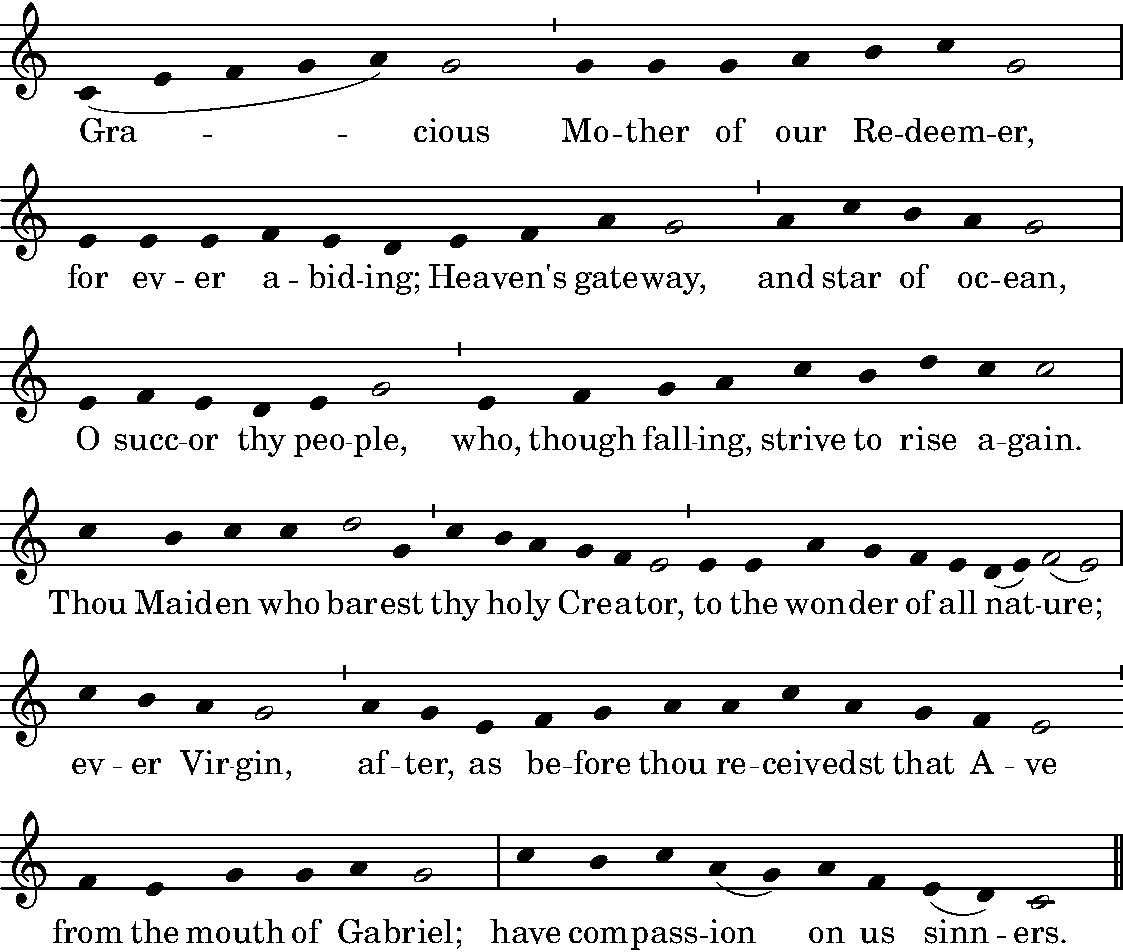
\includegraphics[width=\linewidth]{antiphons/almaredem-crop.pdf}

\instruct{In Advent}

\begin{tabularx}{\linewidth}{lX}
  \textit{Officiant} & The Angel of the Lord announced unto Mary. \\
  \textit{People} & \textbf{And she conceived by the Holy Ghost.}\\
  \textit{Officiant} & Let us pray:
\end{tabularx}

We beseech thee, O Lord, pour thy grace into our hearts: that, as we
have known the incarnation of thy Son Jesus Christ by the
message of an angel, so by his cross and passion we may be
brought unto the glory of his resurrection. Through the same Christ
our Lord.

\begin{tabularx}{\linewidth}{lX}
  \textit{People} & \textbf{Amen.}
\end{tabularx}

\newpage
\instruct{From First Vespers of the Nativity}

\begin{tabularx}{\linewidth}{lX}
  \textit{Officiant} & After Childbearing, O Virgin, thou didst
  remain inviolate. \\
  \textit{People} & \textbf{Intercede for us, O Mother of God.}\\
  \textit{Officiant} & Let us pray:
\end{tabularx}

O God, who by the fruitful virginity of Blessed Mary hast bestowed
upon mankind the reward of eternal salvation: Grant, we beseech thee,
that we may know the help of her intercession through whom we have
been accounted worthy to receive the Author of our life, Jesus Christ
thy Son our Lord.

\begin{tabularx}{\linewidth}{lX}
  \textit{People} & \textbf{Amen.}
\end{tabularx}

\subsection*{Ave Regina caelorum}

\instruct{From Candlemas to Maundy Thursday}

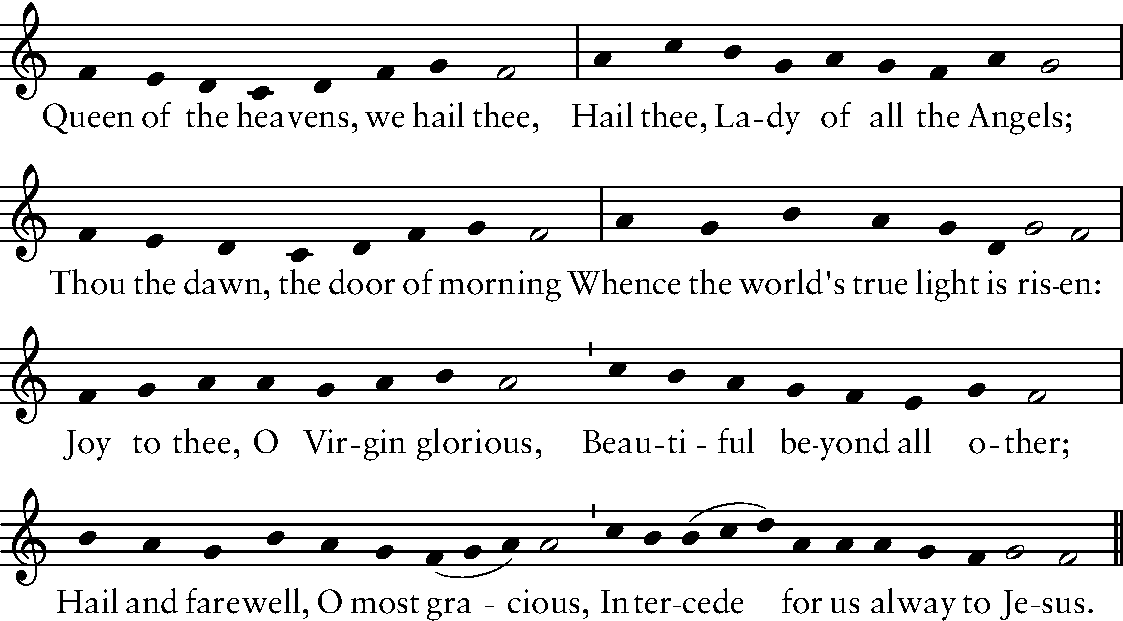
\includegraphics[width=\linewidth]{antiphons/averegina-crop.pdf}

\begin{tabularx}{\linewidth}{lX}
  \textit{Officiant} & Vouchsafe that I may praise thee, O holy Virgin. \\
  \textit{People} & \textbf{Give me strength against thine enemies.}\\
  \textit{Officiant} & Let us pray:
\end{tabularx}

Grant us, O merciful God, protection in our weakness:
that we who celebrate the memory of the holy Mother of God may,
through the aid of her intercession, rise again from our sins.
Through the same Christ our Lord.

\begin{tabularx}{\linewidth}{lX}
  \textit{People} & \textbf{Amen.}
\end{tabularx}

\subsection*{Salve Regina}

\instruct{From First Vespers of Trinity Sunday to Advent}

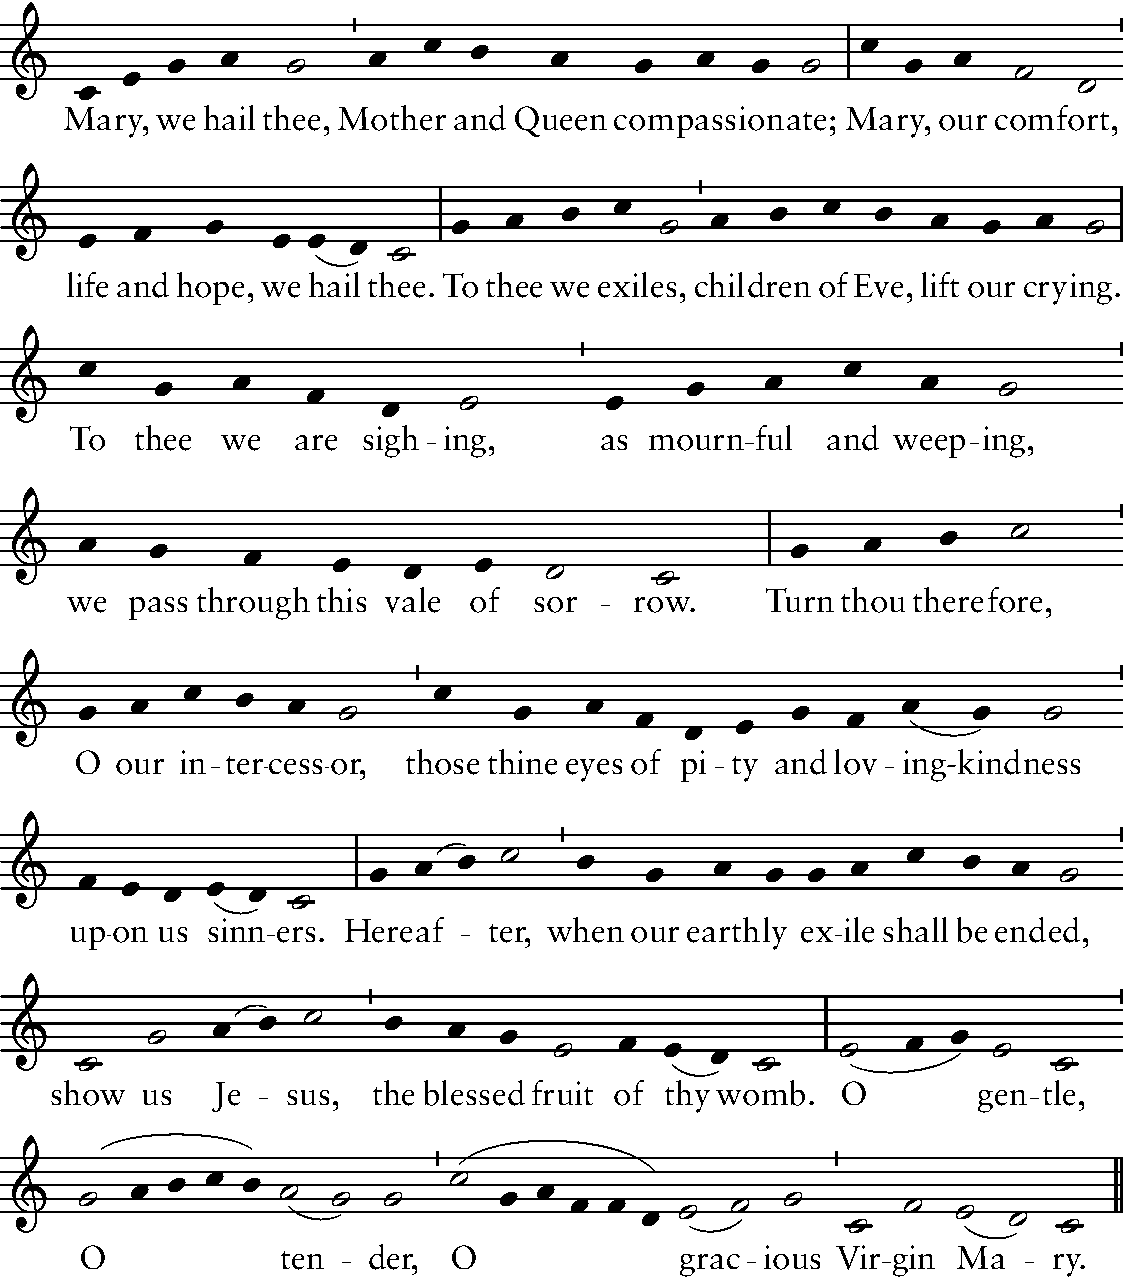
\includegraphics[width=\linewidth]{antiphons/salveregina-crop.pdf}

\newpage
\begin{tabularx}{\linewidth}{lX}
  \textit{Officiant} & Pray for us, O holy Mother of God. \\
  \textit{People} & \textbf{That we may be made worthy of the
  promises of Christ.}\\
  \textit{Officiant} & Let us pray:
\end{tabularx}

Almighty and everlasting God, who by the cooperation
of the Holy Ghost, didst prepare the body and soul of the glorious
Virgin Mother Mary to become a habitation meet for thy Son: Grant
that as we rejoice in her commemoration, we may be delivered by her
loving intercession from our present evils and from eternal death.
Through the same Christ our Lord.

\begin{tabularx}{\linewidth}{lX}
  \textit{People} & \textbf{Amen.}
\end{tabularx}

\end{document}
